% \begin{savequote}[75mm]
% Does this shit even work?
% \qauthor{A Tired Grad Student}
% \end{savequote}

\chapter{High-throughput behavior in rats}
\newthought{The laboratory rat \textit{Rattus norvegicus}} was the first mammalian species domesticated for scientific research\cite{Jacob199}, and has since been the most widely studied specie in biomedical research. In the lab, rats can be trained to perform cognitively demanding tasks. They have a long history as laboratory models for the behavioral study of cognitive capacities, including decision-making\cite{Brunton2013, Raposo2012, Miller2017TwoStep, Piet2018RatsEnvironment}, working memory\cite{Bratch2016}, and spatial navigation\cite{OKeefe1971, Whishaw1995, Aronov2014}. 

One of the most widely used tools for studying animal behavior in the lab is the operant conditioning chamber. With the conditioning chamber, the experimenter gradually shapes the animal's behavior until the desired task is learned. Like most rodent behavior experiments, tests of visual object recognition rely on operant conditioning. Technological developments over the past ten years have enabled experiments to use these traditional conditioning boxes in computer-controlled systems that allow for automated and high-throughput training. 

Automated training methods are more efficient because they require little to no hands-on involvement from the experimenter. Animals can be placed into chambers by staff who are unbiased about the particular study's goals or they can simply live in the boxes with automatically or remotely controlled training regimes\cite{Qiao2018, Poddar2013, Miller2017Twostep}. Thus, high-throughput systems not only allow for more systematic and less biased experiments, but importantly, they also allow many animals to be trained and studied in parallel. Higher-throughput studies provide statistical power difficult to achieve with small-scale animal cohorts and importantly, have the potential to provide a readily available source of animals for physiological access or perturbation studies. These advantages are particularly important for behavioral tasks that are complex and require long training schedules.

In 1930, Karl Lashley\cite{Lashley1930} described a wide range of visual behaviors in rats using what is now a classic two-choice paradigm\ref{fig:FIG?}. In his version of the rig, Lashley tested rats' visual shape recognition capacities by training them to select a particular gate or door depending on what stimulus it showed in order to access a hidden food reward. Fast-forward $\sim$80 years, experiments have relied on similar training rigs to test rats on visual object recognition tasks\cite{Zoccolan2009, ETC}. While most studies using monkeys rely on about 2-3 animals standard rat vision studies use ~4-6 animals per experiment\cite{Vermaercke2012, Tafazoli2012Transformation-TolerantPriming}

In contrast, several groups studying rats outside of traditional visual neuroscience have pushed the bounds to demonstrate the power of high-throughput rat behavior. Of note, Brody and colleagues use highly complex tasks that take rats months to learn, and have developed massively high-throughput behavior systems that train many rats in parallel on various acoustic decision-making and working memory tasks\cite{Miller2017TwoStep, Brunton2013RatsFrom}. In motor skill learning, Olveczky and colleagues have built high-throughput, fully-automated systems for home-cage training\cite{Poddar2013}. In mice, a growing number of high-throughput systems now exist\cite{Qiao2018}). Inspired by the power of large-scale behavior systems, our goal was to take existing visual behavior paradigms in rats and adapt them for high-throughput, automated training. 

% This is a math equation that can go here for now.
% $$\zeta = \frac{1039}{\pi}$$

% %%%%%%%%%%%%%%%%%%%%%%%%%%%%%%%%%%%%%%%%%%%%%%%%%%%%%%%%%
% Results
% %%%%%%%%%%%%%%%%%%%%%%%%%%%%%%%%%%%%%%%%%%%%%%%%%%%%%%%%%
% fig:openratbox
% fig:basic_training
% fig:behavior_generalization

% ---------------------------------------------------------
% OpenRatBox -- the hardware.
\section{OpenRatBox: An open-source platform for high-throughput behavior}
Our approach was to design a visual behavior system that was reproducible, low-cost, and modular. It was critical to design training boxes that would be straightforward to reproduce, not only to maintain constancy from one box to the next, but also to facilitate widespread use both within the lab and across labs. Systematization across research groups can be immensely powerful, especially for studying highly complex, multi-modal processes like decision-making, as exemplified by the International Brain Laboratory\cite{IBL} and the Allen Brain Institute\cite{REFREF}.

In order to build behavior boxes at a larger scale, we relied on low-cost, readily accessible components and open-source software for experimental control. While it is possible to build a highly sophisticated and customized apparatus that meets the particular demands of a given experiment, it can be extremely costly and hard to adapt for other experiments or impossible to use by other labs. In contrast, designing a low-cost system that relies on open-source technology allows it to be more accessible as a tool that can benefit others, while also allowing for continued improvements and new adaptations. 

Modularity is important because a given behavior can be tested under different regimes. For example, two commonly used behavior choice paradigms are Go/No-Go (GNG) and two-alternative forced choice (2AFC) tasks. These paradigms offer different advantages and disadvantages (see X), and also have different hardware requirements. GNG just requires one choice manipulandum, while 2AFC requires at least two.

% FIGURE 1.1 OpenRatBox Schematic
\begin{figure}[t!]
    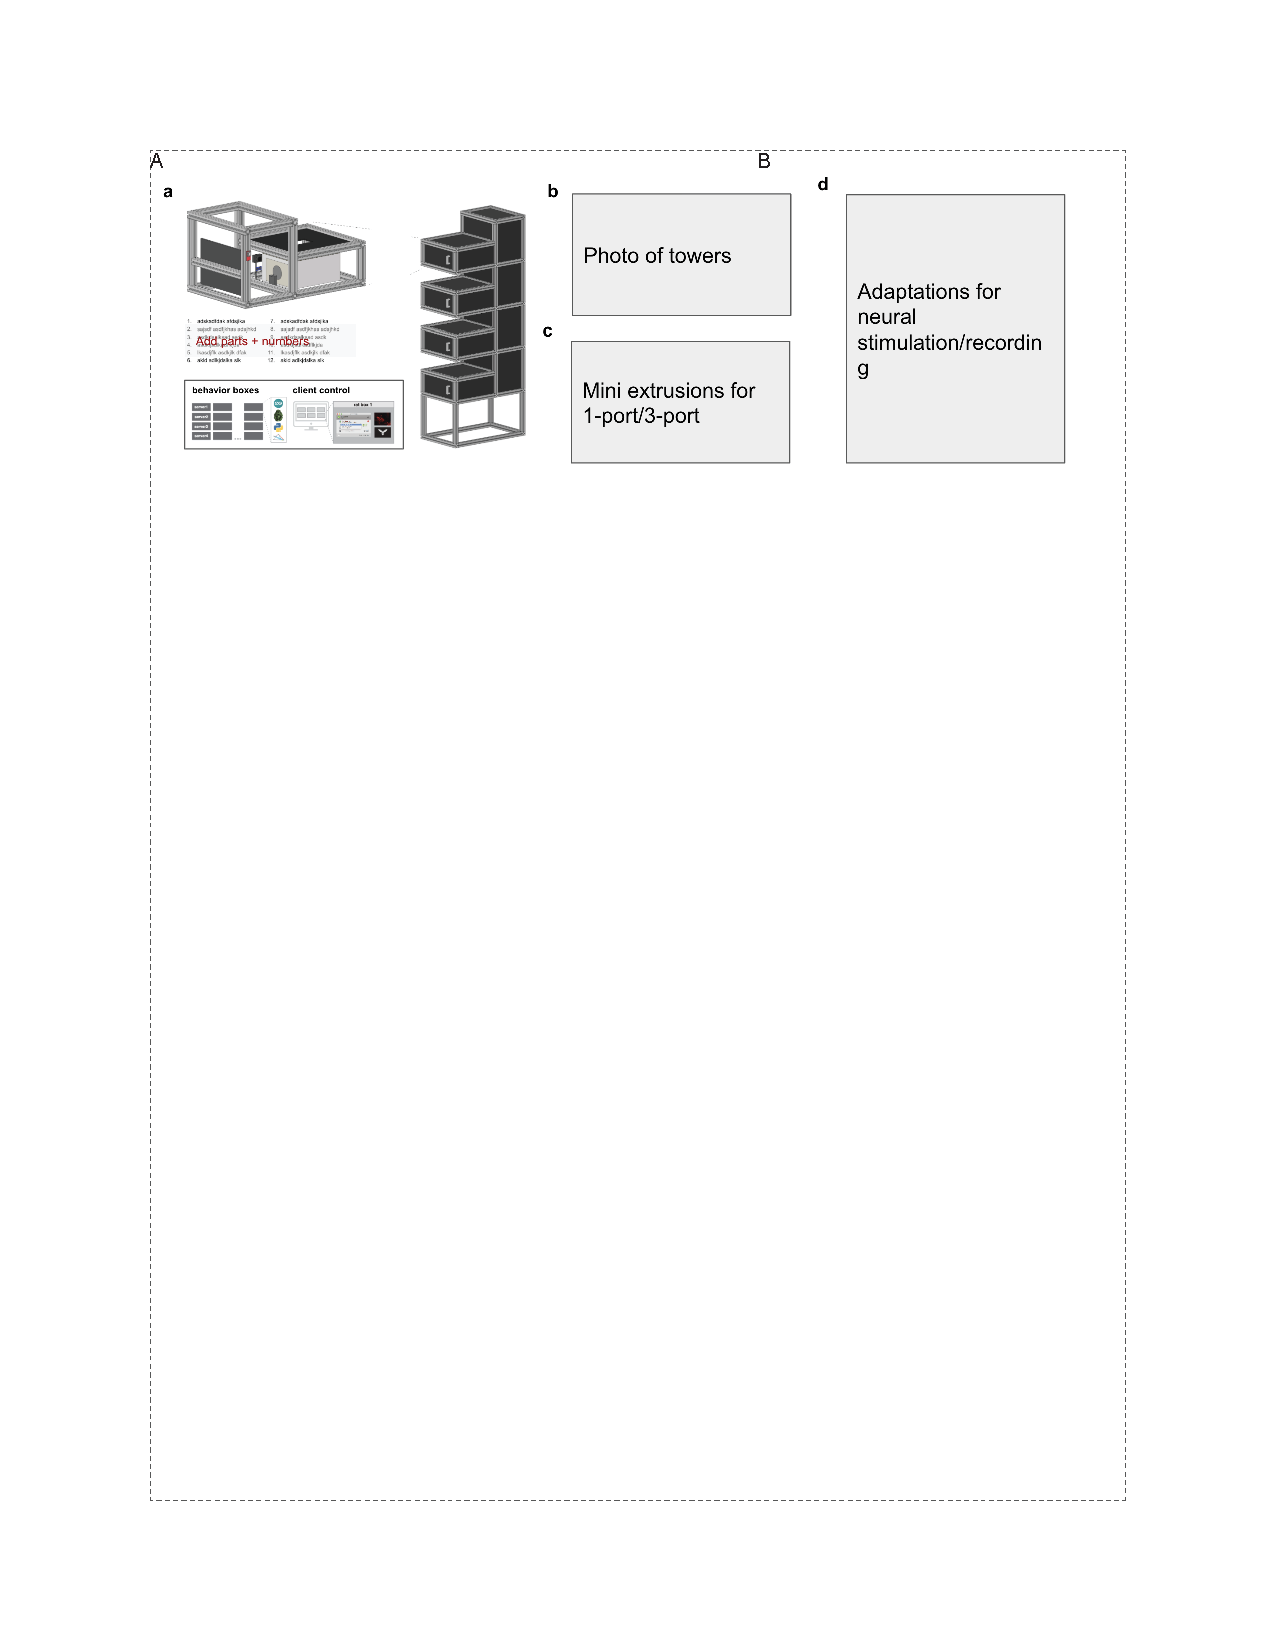
\includegraphics[width=\textwidth]{figures/chapter_1/fig_1-1_openratbox/fig_1-1_openratbox.pdf}
    \vspace{.1in}
    \caption[OpenRatBox]{OpenRatBox: Open-source, automated, high-throughput training. \textbf{A.} Top, Schematic of one training box. Numbers denote relevant parts. Bottom inset, Logic of experimental control: an independent server on each box (here, showing 4 boxes per tower, with a total of 5 towers used for the present study) runs a specified experiment, and a main control computer with a client allows full control of each box. Left, A full tower assembly of four identical training boxes. \textbf{B.} A view of a room of towers used to train the animals in the present work. \textbf{C.} Plug-and-play components can be swapped out for different task paradigms. \textbf{D.} Boxes equipped with a commutator can house tethered animals for chronic neural stimulation or recording experiments.  
    \label{fig:openratbox}}
\end{figure}

The overall design of each box is identical, and experiment-specific adjustments are made with modular components. The main vestibule of each unit houses the animal's cage and all hardware needed to collect the animal's response and monitor its behaviors (Figure\ref{fig:openratbox}\textbf{A}). Each unit is equipped with a small computer that allows as many experiments to be run independently and in parallel as there are boxes. The external frame is composed of aluminum extrusion bars and custom-cut acrylic paneling that fits into the railing slots of the bars, such that an arbitrary number of boxes can be built on top of the next, limited by the available vertical space. In our behavior rooms, we had enough space for towers composed of 4 stacked units (Figure\ref{fig:openratbox}\textbf{B}). All the training boxes are controlled and monitored by a control computer that runs a client (MWorks) that interfaces with the servers running in each behavior box. 

Within a given unit, there are two partitions. The monitor is mounted on a partition separate from the main vestibule in order to keep it clean and protected (for example, from chewing, or stray water droplets and bedding). The animal has visual access to the monitor through a window separating the monitor from the main vestibule that holds the cage. The cage itself is held in place with two spring-loaded latches that allow the cage to be loaded into the same relative position, if necessary. The cage locking mechanism was adapted from a commercially available, self-standing animal cage rack, in which each cage is locked into the air circulation and filtration system. The box is thus designed to support fully live-in animal behavior training. 

During visual behavior sessions, the animal has access to the reward ports and monitor through a small window placed at one end of the home cage. In the case of live-in training, the window can be gated shut during non-training times, if desired. Mini extrusion bars (REFREF) are screwed directly into the acrylic floor of the main vestibule around the animal's access window. This effectively creates a mountable rail system for attaching experiment-specific components, such as reward ports, USB cameras, and IR detectors (Figure\ref{fig:openratbox}\textbf{C}). As such, any modifications specific to a paradigm (\textit{e.g.}, one reward port or three reward ports) could be easily attached or removed from one box to the next. All wiring feeds through small access holes cut into the acrylic pieces embedded into the extrusion bars, as does tubing for water delivery of rewards. Attached to each box is a small computer (Mac Mini, though others are possible) that runs the experiment (visual stimulation, I/O control, and so on). 

Finally, the entire system can be equipped for neural stimulation and recording in tethered rats. The spacing between the stacked boxes creates sufficient room for a commutator system that carries a cable from the animal's head through a hole in the acrylic ceiling of the main vestibule (Figure\ref{fig:openratbox}\textbf{D}). Though we tested both Go/No-Go and two-choice behavior paradigms, we selected the latter for the remainder of our behavior studies (see Discussion) as this is a well-established paradigm used to test visual object recognition behavior in rats\cite{Lashley1930, Zoccolan2009, Prusky2000, REFREF}. 

% ---------------------------------------------------------
% OpenRatBox -- the functionality (high-throughput training)
\section{High-throughput behavior training}
We trained rats to perform a simple, two-category object discrimination task\cite{Zoccolan2009} (Figure\ref{fig:basic_training}\textbf{A}). This is a three-port paradigm in which rats lick the center port to initiate trials, and one of the two flanking ports to indicate which object is on the screen. Rats initiated each trial by licking the middle of three capacitive lick ports, which triggered the appearance of one static visual object (1 of the two object categories) on the screen (see Methods for details). The rats indicated which visual object was present by licking one port, \textit{e.g.}, the left port, for object A, and the other \textit{e.g.}, for object B, with stimulus-port mappings counterbalanced across animals (Figure\ref{fig:basic_training}\textbf{B}).

% FIGURE 1.1 Basic training
\begin{figure}[t!]
    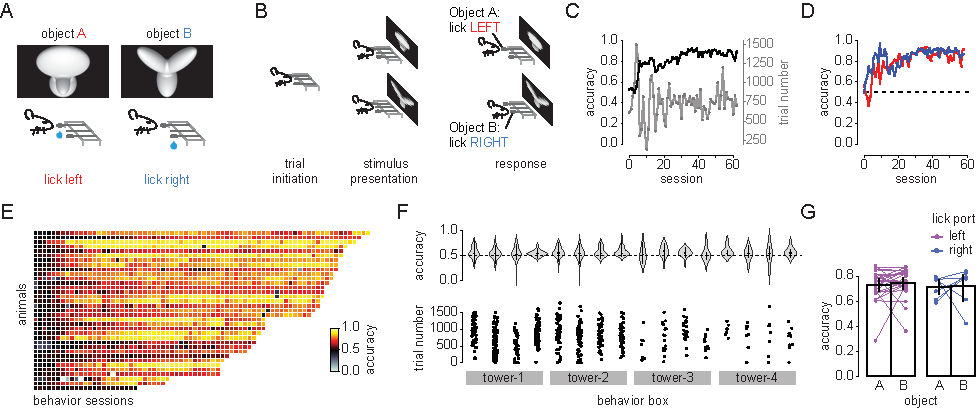
\includegraphics[width=\textwidth]{figures/chapter_1/fig_1-2_basic_training/fig_1-2_basic_training.pdf}
    \vspace{.1in}
    \caption[High-throughput training]{High-throughput training on a simple two-alternative choice task. \textbf{A.} Logic of the basic, two-category object discrimination task. \textbf{B.} Trial structure. \textbf{C.} Example training data from one rat. Black, overall accuracy as a function of training session number. Gray, Number of trials completed in each session. \textbf{D.} Accuracy for each of the two objects for the example rat shown in \textbf{C}. \textbf{E.} Overall accuracy for a large cohort of animals (N=33 rats) as a function of training session. \textbf{F.} Top, Accuracy for each box and each tower. Each group, indicated by brackets, represents one tower of 4 boxes (4 towers shown), with the leftmost group of points corresponding to the highest box, and the rightmost points. Bottom, Number of trials performed per session for each box and tower. Notation as in the upper panel. \textbf{G.} Performance split by stimulus-port mapping and object identity. Red, accuracy for object A. Blue, accuracy for object B. Portmap 1 and 2 denote whether the animal is assigned to lick port 1 for object A or port 2 for object A, and vice versa.
    \label{fig:basic_training}}
\end{figure}

Animals could be trained to perform shape discriminations for reasonably dissimilar objects in one month or less, and readily performed several hundred trials per day in the automated training rig (Figure\ref{fig:basic_training}). Importantly, overall behavior metrics were similar across all behavior box units and towers. We observed no differences in overall accuracy, accuracy by port assignment, or number of trials completed per session. Almost all rats reached criterion for the appropriate stimulus-port pairing within REFREF sessions (Figure\ref{fig:basic_training}). Trained rats performed with high accuracy for both objects (average REFREF +/- std, n=32/34 rats reached criterion performance of 70\% correct across REFREF +/- STD sessions). These results demonstrate that our behavior units are reproducible and successful for training large cohorts of animals. 

% ---------------------------------------------------------
% Behavior Generalization
\section{Visual object recognition behavior}
Previous studies have demonstrated that rats are capable of recognizing never-before-seen views of objects familiar objects\cite{Zoccolan2009, Vermaercke2012, Tafazoli2012Transformation-TolerantPriming, REFREF}. Our goal was to validate that rats will perform these behaviors in our high-throughput system. Using OpenRatBox, we tested how rats generalize across two types of transformations: the first was a psychophysical test, by which we identified rats’ discrimination thresholds separating one object from another, and the second was an invariant recognition test, where rats had to discriminate objects across changes in particular views (Figure\ref{fig:behavior_generalization}). 

Once rats reliably discriminated between the two objects, we then tested on their ability to generalize across two types of transformations. To identify perceptual discrimination thresholds separating the two objects, we tested identity-changing transformations in which images were parametrically varied between the two original objects at a given view.

% FIGURE 1.3 Behavior generalization.
\begin{figure}[t!]
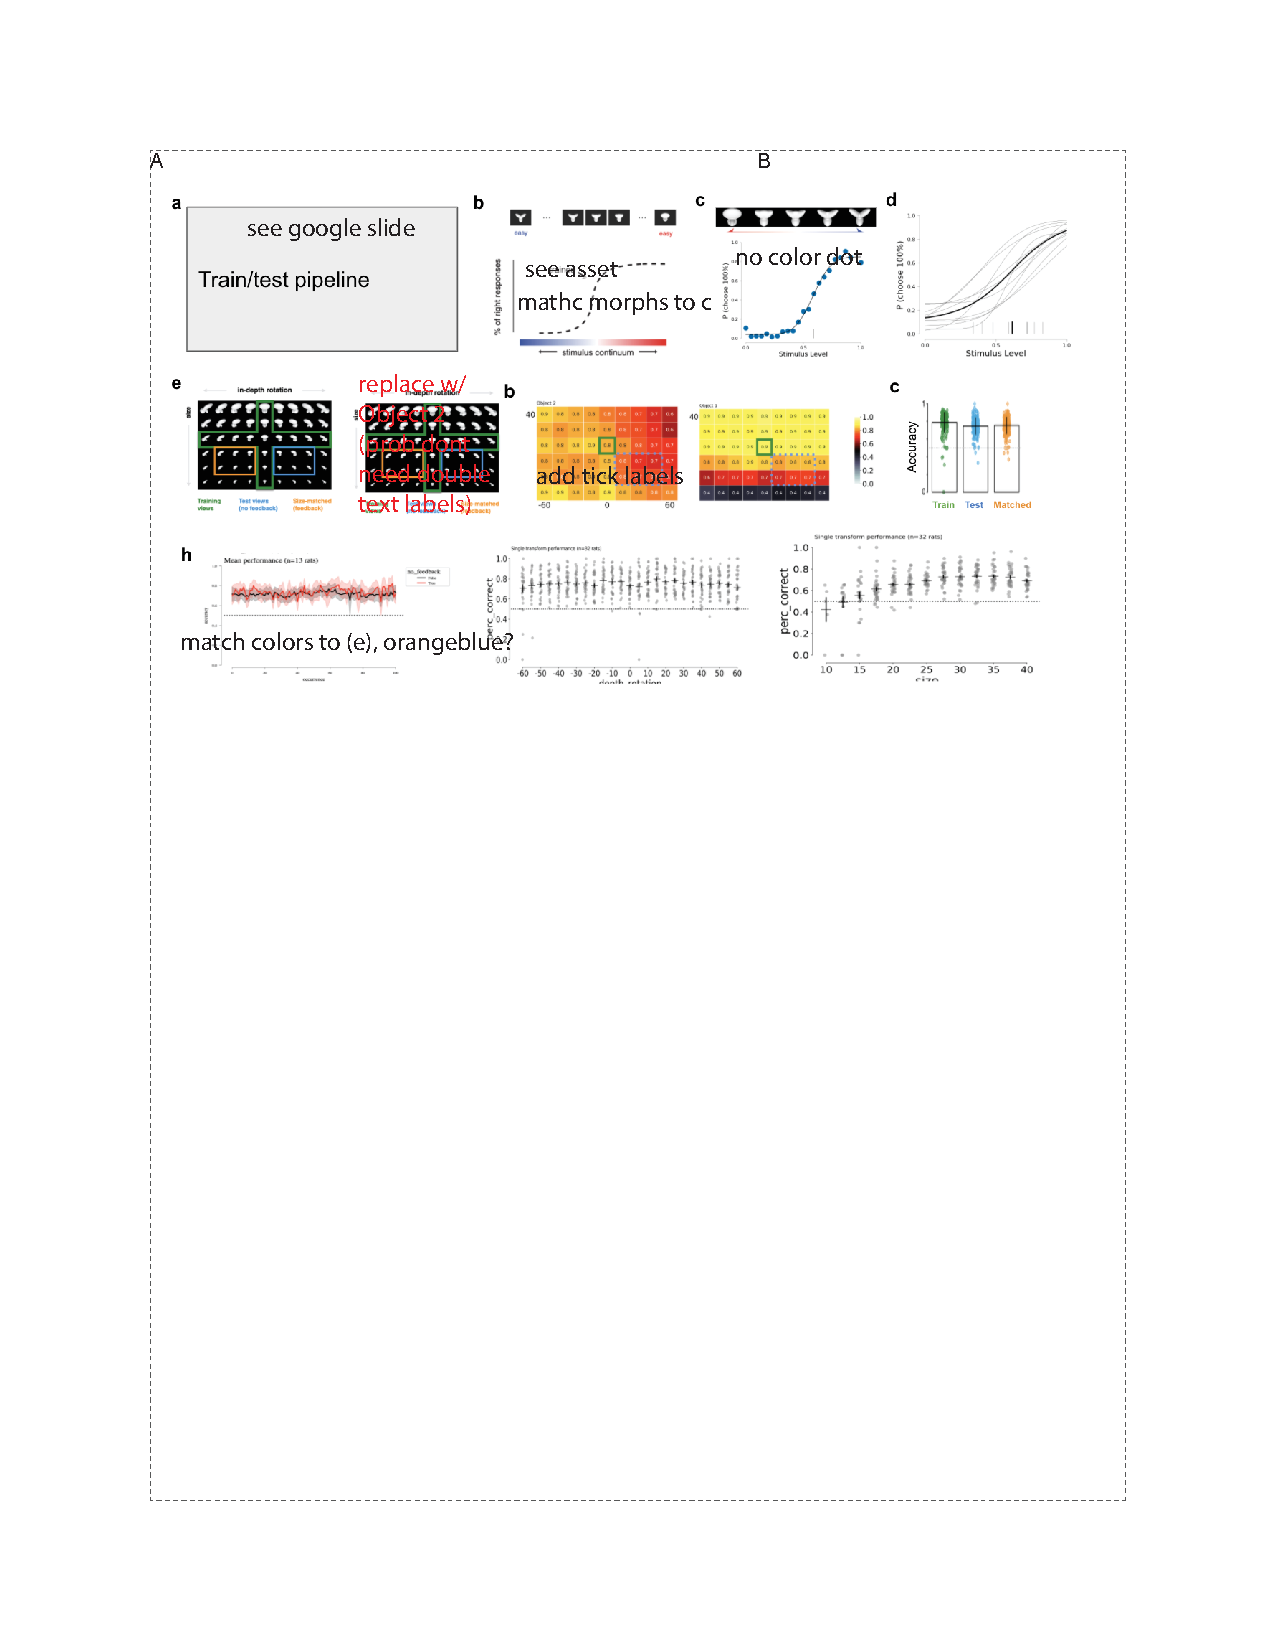
\includegraphics[width=\textwidth]{figures/chapter_1/fig_1-3_behavior_generalization/fig_1-3_behavior_generalization.pdf}
    \vspace{.1in}
    \caption[Generalization of visual behavior]{Generalization to identity-preserving and identity-changing transformations. \textbf{A.} Training and testing pipeline. Animals are first trained on the basic discrimination task. Those that pass criterion performance are then tested on identity-changing or identity-preserving generalizations on probe trials that are interleaved with the basic task. \textbf{B.} Morph stimuli create an axis along which identity changes across a stimulus continuum between the original anchors, object A and B. \textbf{C.} Example data on the morph probe trials for one rat. Dots, average across trials for each morph level. Line, fit psychometric curve. \textbf{D.} Pyschometric curves for one cohort (N=10 rats). Thin lines, individual rats. Thick line, average psychometric curve across rats. \textbf{E.} Identity-preserving transformations tested for each of the original objects: 6 sizes and 9 in-depth rotations. Green, subset of conditions used for training. Blue, test transformations for which feedback was never provided. Orange, size-matched (\textit{i.e.}, acuity-matched) transformations of the test views, but for which feedback was provided, to compare the effect of feedback on generalization performance. No-feedback quadrants were counterbalanced across animals. \textbf{F.} Example rat. \textbf{G.} Accuracy for rats in one cohort (n=10 rats) for train views, test views, and size-matched feedback views. Colors as in \textbf{E}. Each circle denotes session accuracies for a given rat, all rats shown. Error bars, SD. \textbf{H.} Accuracy as a function of the N-th presentation of a given transformation for feedback-provided (REFREF color) and no-feedback (REFREF color) conditions. Shading, SD across animals. \textbf{I.} Accuracy for each depth-rotation tested. Each dot is the session accuracy for a given rat. Lines, mean and SD across sessions. \textbf{J.} Same as \textbf{I}, but for each stimulus size tested. 
    \label{fig:behavior_generalization}}
\end{figure}
%     \caption*{\textbf{Figure 2.1} Example figure and tips -- A) Your figure numbers should follow the format of Figure chapter#.figure#. B) Set width equal to textwidth. C) Specify position as [t!] to insert at page top.}
% \end{figure}

Specifically, we created a shape continuum by generating a series of morphs that varied along a high-dimensional identity axis separating the two original objects (as shown in Figure\ref{fig:morphs}). The identity axis was defined in N-dimensional pixel space, and morphs were selected to evenly sample distances along this axis (see Methods). We then tested the extent to which linear similarity in pixel space reflected perceived similarity in rats trained to discriminate the two anchor objects. 

Rats were presented with a morph image on a small fraction of trials (<15\%, see Methods) during the ordinary discrimination task. No feedback was provided on these probe trials in order to measure perceived, rather than trained, perceptual judgements. These probe trials were then used to build up a psychophysical curve to determine the animals' naive behavior in classifying the objects as ``A'' or ``B''. We fit a psychometric curve to the probe trials using maximum likelihood estimation (psignifit4, REFREF, see Methods). These curves characterize the category boundary along the morph axis. We found that that rats perceptual choices matched the physical similarity of the morphed objects, though there was individual variation across rats (slope, REFREF +/- ; threshold, REFREF +/- SEM; lapse rate, REFREF +/- SEM, across n=10 rats). 

% FIGURE 1.3 INVARIANCE TEST
To test how well animals discriminate objects across shape changes that preserve object identity, we tested the same rats on an object recognition task. Consistent with previous studies\cite{Zoccolan2009, Tafazoli2012Transformation-TolerantPriming, REFREF}, we found that performance generalized robustly across identity-preserving transformations, such as changes in size and in-depth rotation (Figure\ref{fig:behavior_generalization}\textbf{e}). Importantly, accuracy was high on test trials (~80\% accuracy, mean REFREF +/- std, n=REFREF rats), where animals never received feedback (Figure\ref{fig:behavior_generalization}\textbf{F-G}), demonstrating that performance on novel views was spontaneous, rather than learned. In fact, accuracy was high across all presentations of novel views, with or without feedback (Figure\ref{fig:behavior_generalization}\textbf{H}). These results demonstrate that rats are capable of true generalization, and are not simply learning stimulus-response pairings. 

% ---------------------------------------------------------
% Closing remarks
% \section{Discussion?}
High-throughput behavior is important for practical reasons, but also scientific ones. 
Standardization is important. 

We found that rats readily perform hundreds of trials per day in our behavior system and learn difficult visual tasks in 2-3 weeks. We use OpenRatBox to show that rats robustly generalize to novel views of objects, i.e., across identity-preserving transformations, and make perceptual choices that follow our morph axis of identity transformations. While similar behavioral results have been shown previously\cite{Zoccolan2009, Tafazoli2012Transformation-TolerantPriming, Vermaercke2012}, here, we demonstrate that a) we can replicate these results with our high-throughput behavior system, and b) in response to our particular stimuli, rats respond correctly in the absence of training on the transformations (no feedback conditions and morph probe trials). We will use the same stimuli when characterizing neural representations in naive rats in a later chapter. 

% In Go/No-Go (GNG) paradigms, the animal responds to a given stimulus (the "Go" condition) by licking a choice port or pressing a lever, and must withhold a response otherwise (the "No-Go" condition). GNG paradigms have fewer moving parts, requiring only one response type, which can make it easier to learn. However, subjects tend to make more Go responses in the GNG task, as the Go response is rewarded while other other behaviors are not\cite{REFREF}. 

% For physiology experiments, GNG paradigms are more amenable to head-restrained animals, since the animal only needs to make one type of response. On the other hand, since reward strongly modulates neural activity, and GNG paradigms can be challenging as the stimulus, response, and reward are tightly linked\cite{REFREF}. Multi-port tasks, like two-choice paradigms, overcome many of these drawbacks, as the animal is trained to respond in one way to condition A and some other way to condition B. In this way, the stimulus, response, and reward can be disentangled, but at the cost of a more complicated task structure that can make interpretations difficult in still other ways. However, they can be more difficult to adapt for head-restrained conditions. Animals normally use head movements or their whole body to reach one reward port or the other\cite{REFREF}, which is not possible in physiology experiments that require the animal's head to be fixed in place in the recording apparatus. 


% \texttt{This is a line of code.}


% For an example of a full page figure, see Fig.~\ref{fig:myFullPageFigure}.

% % EXAMPLE FIGURE 
% \begin{figure}[t!]
%     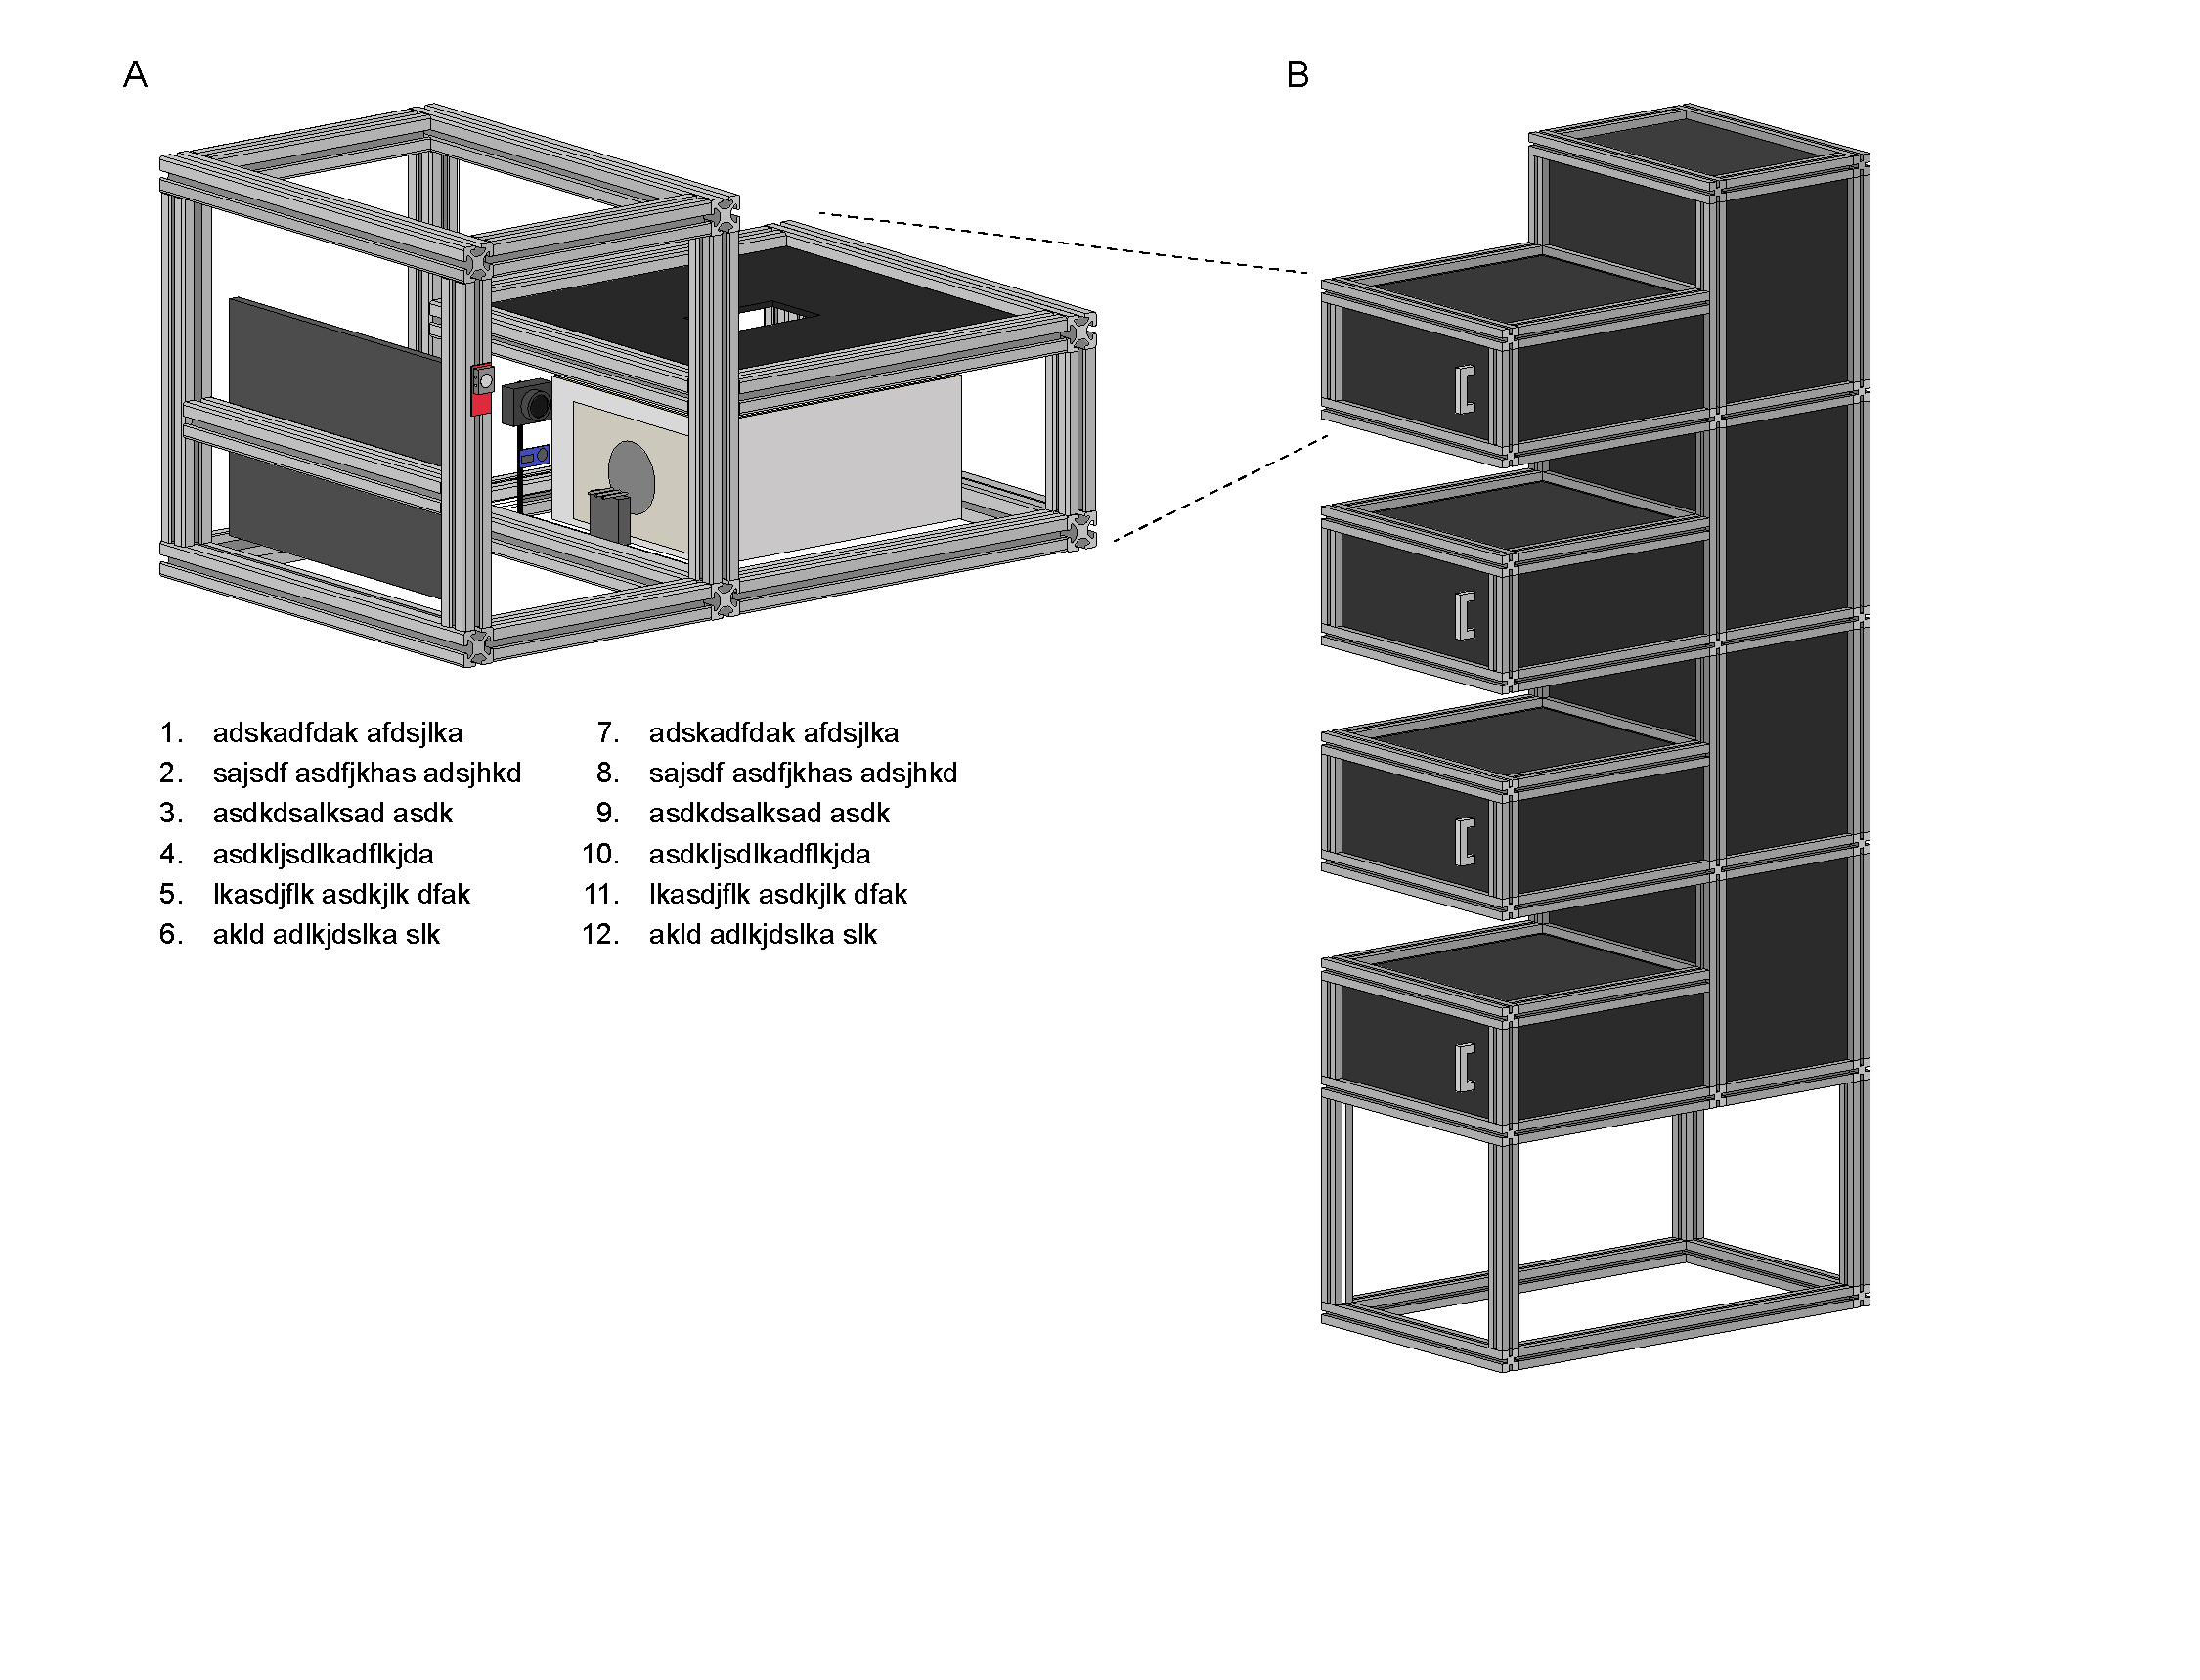
\includegraphics[width=\textwidth]{figures/chapter_1/ratbox_schematic.pdf}
%     \vspace{.1in}
%     \caption*{\textbf{Figure 2.1} Example figure and tips -- A) Your figure numbers should follow the format of Figure chapter#.figure#. B) Set width equal to textwidth. C) Specify position as [t!] to insert at page top.}
% \end{figure}

%% Requires fltpage2 package
%%
% \begin{FPfigure}
% 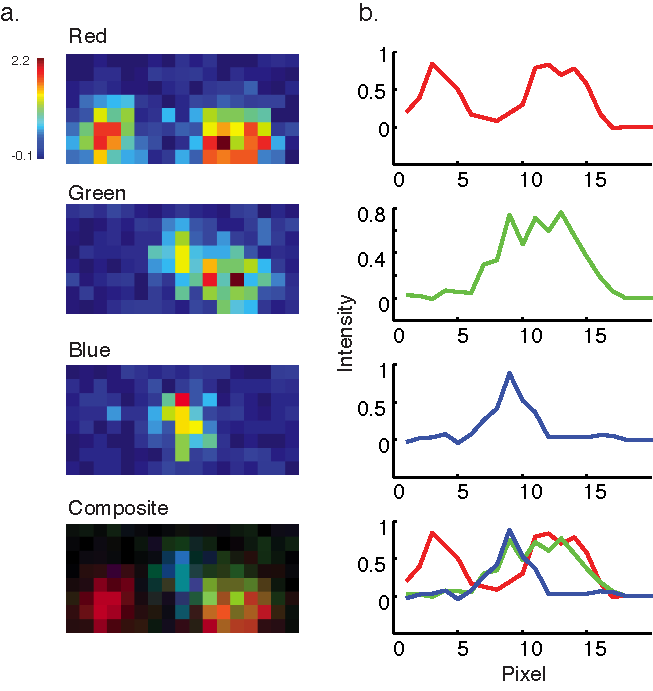
\includegraphics[width=\textwidth]{figures/fullpage}
% \caption[Short figure name.]{This is a full page figure using the FPfigure command. It takes up the whole page and the caption appears on the preceding page. Its useful for large figures. Harvard's rules about full page figures are tricky, but you don't have to worry about it because we took care of it for you. For example, the full figure is supposed to have a title in the same style as the caption but without the actual caption. The caption is supposed to appear alone on the preceding page with no other text. You do't have to worry about any of that. We have modified the fltpage package to make it work. This is a lengthy caption and it clearly would not fit on the same page as the figure. Note that you should only use the FPfigure command in instances where the figure really is too large. If the figure is small enough to fit by the caption than it does not produce the desired effect. Good luck with your thesis. I have to keep writing this to make the caption really long. LaTex is a lot of fun. You will enjoy working with it. Good luck on your post doctoral life! I am looking forward to mine. \label{fig:myFullPageFigure}}
% \end{FPfigure}
% \afterpage{\clearpage}

